% \documentclass{article}
\documentclass[journal]{IEEEtran}
\usepackage{amsmath,amsfonts}
\usepackage{algorithmic}
\usepackage{algorithm}
\usepackage{array}
\usepackage{graphicx}
\usepackage[caption=false,font=normalsize,labelfont=sf,textfont=sf]{subfig}
\usepackage{textcomp}
\usepackage{stfloats}
\usepackage{url}
\usepackage{verbatim}
\usepackage{cite}
\usepackage{color,soul}
\usepackage{lipsum}
\usepackage{pgfplotstable}
\usepackage{booktabs}
\usepackage{multirow}
\hyphenation{op-tical net-works semi-conduc-tor IEEE-Xplore}
% updated with editorial comments 8/9/2021

\begin{document}

\title{Size-Adaptive Density Estimation for Accurate Object Counting in Dense Environments}

\author{\IEEEauthorblockN{Phu Nguyen\IEEEauthorrefmark{1},
                An Nguyen Duc\IEEEauthorrefmark{2},
                Bao Bui Quoc\IEEEauthorrefmark{1}}\\
        \IEEEauthorblockA{\IEEEauthorrefmark{1}Department of Electronics, Ho Chi Minh University of Technology (HCMUT), Vietnam National University-Ho Chi Minh City (VNU-HCM), Ho Chi Minh City, Vietnam}\\
        \IEEEauthorblockA{\IEEEauthorrefmark{2}..., ..., ...}
        % <-this % stops a space
        \thanks{This paper was produced by the IEEE Publication Technology Group. They are in Piscataway, NJ.}% <-this % stops a space
        \thanks{Manuscript received April 19, 2021; revised August 16, 2021.}}

% The paper headers
\markboth{Journal of \LaTeX\ Class Files,~Vol.~14, No.~8, August~2021}%
{Shell \MakeLowercase{\textit{et al.}}: A Sample Article Using IEEEtran.cls for IEEE Journals}

% \IEEEpubid{0000--0000/00\$00.00~\copyright~2021 IEEE}

% Remember, if you use this you must call \IEEEpubidadjcol in the second
% column for its text to clear the IEEEpubid mark.

\maketitle

\begin{abstract}
        Object counting in images with significant size variations and dense object clusters remains a challenge in computer vision. Existing methods often struggle with accuracy due to limitations in handling these complexities. This paper proposes an approach based on a Size-Adjustable Gaussian Kernel for density map generation, addressing the issue of object size heterogeneity. Our method dynamically adjusts the kernel parameters based on individual object dimensions, ensuring accurate representation of both spatial distribution and size variations. We utilize a modified VGG16 architecture with a Bi-directional Feature Pyramid Network (BiFPN\cite{bifpn}) and attention mechanisms (ECA\cite{eca} and MSCA\cite{msca}) for robust feature extraction and object recognition across scales. Extensive experiments on a challenging shrimp larvae image dataset demonstrate the superior performance of our method, achieving significant improvements in counting accuracy compared to state-of-the-art approaches. This work paves the way for more precise and reliable object counting in various applications with diverse object sizes and densities.
\end{abstract}

\begin{IEEEkeywords}
        Object counting, density estimation, size-adjustable Gaussian kernel, deep learning, convolutional neural networks, attention mechanisms, shrimp larvae, aquaculture.
\end{IEEEkeywords}

\section{Introduction}
Object counting within images forms a crucial task in various domains, from crowd analysis and traffic monitoring to ecological surveys and industrial quality control. However, achieving accurate counts, especially when objects exhibit significant size variations and appear in dense clusters, presents a persistent challenge in computer vision. Existing methods often fall short due to inherent limitations in handling these complexities.

Detection-based approaches\cite{shrimp_yolo1,shrimp_yolo2,yolo3, det1, shrimp_det2, shrimp_rcnn1,shrimp_rcnn2,rcnn3}, while effective for well-defined and separated objects, struggle with accuracy in dense scenarios where objects overlap. The reliance on precise bounding boxes becomes problematic, leading to miscounts and inaccurate localization. Similarly, regression-based methods\cite{shrimp_seg1,shrimp_seg2,shrimp_seg3,shrimp_seg4,shrimp_seg5,shrimp_seg6}, while offering a direct mapping from image features to object counts, often overlook crucial spatial information, resulting in a loss of detail regarding object distribution and arrangement within the scene.

Density map-based methods have emerged as a promising alternative, leveraging spatial information to generate density maps that reflect the distribution of objects within an image. However, conventional approaches often employ fixed Gaussian filters with constant kernel size and variance, neglecting the inherent size variations among objects. This leads to suboptimal performance, particularly when dealing with populations exhibiting diverse sizes. While some methods attempt to address this by using adaptive Gaussian filters based on average distances between neighboring objects, they still lack the precision achieved by incorporating individual object size information.
To overcome these limitations, this paper presents a novel approach that tackles the challenges of object size variation and density head-on. Our proposed method introduces a Size-Adjustable Gaussian Kernel for generating density maps. This kernel dynamically adjusts its parameters based on the individual dimensions of each object, ensuring that the generated density map accurately reflects both the spatial distribution and the size variations within the object population.

We leverage the power of Convolutional Neural Networks (CNNs) for feature extraction, employing a modified VGG16 architecture as the backbone of our model. This architecture is further enhanced by the integration of a Bi-directional Feature Pyramid Network (BiFPN\cite{bifpn}) to effectively capture multi-scale features, crucial for recognizing objects of varying sizes. Additionally, we incorporate attention mechanisms, such as Efficient Channel Attention (ECA\cite{eca}) and Multi-Scale Conv Attention (MSCA\cite{eca}), to refine the model's focus on relevant features and improve object recognition across different scales. This comprehensive approach ensures that our model effectively captures the intricacies of object size and distribution within the image.

We validate the effectiveness of our proposed method through extensive experiments on a challenging dataset of shrimp larvae images. The inherent size heterogeneity within this population, coupled with the dense clustering of individuals, makes it an ideal testbed for evaluating our approach. The results demonstrate that incorporating object size information into the density map generation process leads to significant improvements in counting accuracy compared to existing methods. Our Size-Adjustable Gaussian Kernel, in conjunction with the powerful feature extraction and attention mechanisms of our CNN architecture, effectively addresses the challenges posed by diverse object sizes and densities, paving the way for more precise and reliable object counting in various applications.

\section{Related Works}
\subsection{Density Map Generation}
Counting the number of objects in an environment where objects are in dense and overlap each other remains a topic that has been extensively researched, and there are numerous positive solutions proposed to address it. According to Loy \textit{et al}. \cite{loy2013crowd}, they have categorized three primary approaches for tackling this issue: detection-based methods \cite{shrimp_yolo1,shrimp_yolo2,yolo3, det1, shrimp_det2, shrimp_rcnn1,shrimp_rcnn2,rcnn3}, regression-based methods \cite{shrimp_seg1,shrimp_seg2,shrimp_seg3,shrimp_seg4,shrimp_seg5,shrimp_seg6}, and density estimation-based methods \cite{shrimp_density_1, shrimp_density_2, shrimp_density_3, mcnn, sanet, csrnet, cffnet, can, tednet, sfanet, dm, sganet, bayesian}.

Primarily, detection-based methodologies stand out in the quest for object localization within images. These approaches leverage sophisticated object detection frameworks, with a prevailing emphasis on their deployment in early researches. The efficacy of these methods hinges on meticulously trained detection models capable of discerning and extracting comprehensive object features. Prominent instances include the YOLO (You Only Look Once) model \cite{shrimp_yolo1, shrimp_yolo2, yolo3}, as well as the R-CNN (Region-based Convolutional Neural Network) model \cite{shrimp_rcnn1, shrimp_rcnn2, rcnn3}. These models, meticulously trained to identify objects, employ bounding boxes to enumerate objects in images. Nevertheless, their precision exhibits a proclivity to diminish in scenarios where objects are densely clustered or overlap. This phenomenon persists despite the models' adeptness in assimilating information about the objects. As a result, the effectiveness of this approach is most pronounced when the objects to be counted display clear demarcations, introducing challenges in accurately determining bounding box coordinates, especially within densely populated and overlapping object scenarios.\cite{densitymapsurvey}.

To overcome the constraints inherent in detection-based methodologies, regression-based approaches provide a direct mapping from crowd images to numerical object quantities by learning the relationship between extracted features and the actual object count. Despite their success in mitigating challenges related to congestion and overlap, these methods tend to neglect the spatial distribution of objects—an essential factor for precise counting.

The density map-based approach strategically exploits spatial information to formulate density maps for individual training samples, facilitating the computation of the final object count through summation across the density map. This methodology effectively addresses the limitations inherent in regression-based techniques by preserving pertinent spatial details of enumerated objects. Pioneering this paradigm, Lempitsky \textit{et al.} advocate for the conversion of point annotations into density maps via Gaussian kernel filters \cite{firstdensity}. Their subsequent model training involves labels with the density maps generated from these Gaussian filters. The density map-based approach  garnering widespread adoption due to its promising outcomes. However, the judicious selection of Gaussian filter parameters, such as kernel size and variance, remains a pivotal consideration.

While conventional density map methods \cite{firstdensity, shrimp_density_1} often apply a fixed Gaussian filter with the same kernel size and variance parameters across the entire input image, leading to a loss of object size information, advanced strategies strive to overcome this limitation. They employ adaptive Gaussian filters \cite{mcnn, shrimp_density_2, sanet, csrnet, cffnet, can, tednet, sfanet, sganet} that dynamically adjust based on the average distance between neighboring objects, thereby mimicking object sizes within intricate geometric contexts. Nevertheless, these approaches still compromise on the accuracy achieved due to the lack of object size information. Remarkably, models trained using these methods employ loss functions that supervise pixel-to-pixel transitions from input images to density map outputs, emphasizing the crucial role in producing high-quality density maps for optimal performance. Thus, in addition to preservation of spatial information remains a hallmark advantage of density map-based methodologies, the integration of object size information is necessary for crafting superior density maps, thereby augmenting overall model efficacy.
\subsection{CNN-based methods}
Convolutional Neural Networks (CNNs) have emerged as a powerful paradigm, showcasing remarkable efficacy across diverse computer vision applications. Among these, the task of crowd counting in images or videos has particularly benefited from CNN-based approaches. Various strategies within the CNN framework have been explored, including but not limited to multi-column CNN \cite{mcnn, sanet,shrimp_density_2, tednet}, Dilated CNN \cite{csrnet, dadnet, adaptivedilated, spatiotemporaldilated}, and Pyramid Pooling \cite{scalepyramid, atrouspyramid, fpanet}, all geared towards optimizing the extraction and synthesis of input features.

One notable advancement in the realm of multi-column CNNs is the MCNN (Multi-column CNN) model proposed by Zhang \textit{et al.} \cite{mcnn}. This innovative model excels in its ability to extract a spectrum of diverse data features at different scales. Each column within the architecture is adept at learning distinct features, fostering a comprehensive synthesis of information. However, the inherent complexity introduced by employing multiple columns, each dedicated to extracting diverse data, poses a challenge.

In the dilated CNN approach, the CSRNet \cite{csrnet} model has made significant strides by incorporating dilated kernels in various branches. This strategic integration allows for the creation of larger receptive fields, enabling the network to capture more extensive contextual information without imposing an undue burden on system resources.
Another noteworthy approach is exemplified by FPANet model (Zhai \textit{et al.}, 2023) \cite{fpanet}, which strategically amalgamates multi-scale features from a pyramid architecture, effectively addressing challenges arising from scale variations.
The amalgamation of multi-column designs, multi-branch CNN architectures, and pyramid structures in these methods underscores their efficiency in feature extraction across diverse hierarchical levels. Building upon these precedents, our research endeavors to integrate the BiFPN (Bi-directional Feature Pyramid Network) \cite{bifpn} architecture into our neural network. This augmentation is poised to introduce a nuanced, multi-level contextual understanding, specifically tailored to tackle challenges associated with object scale variations—a focal point within the purview of our investigation.
\begin{figure*}[t]
        \centering
        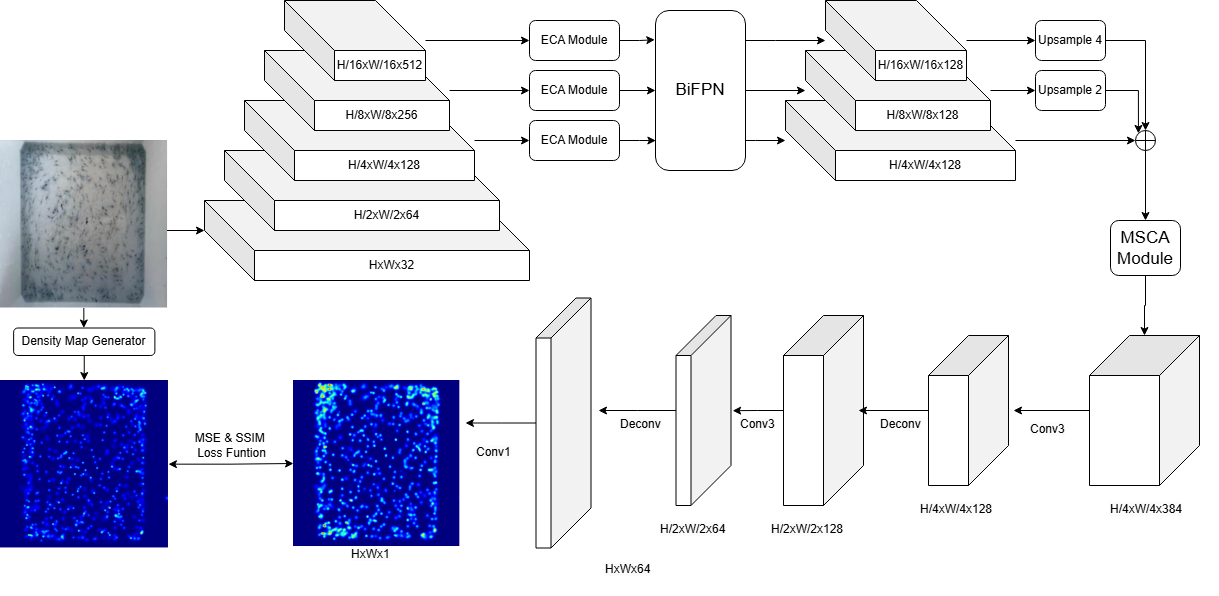
\includegraphics[width=\linewidth]{Fig/model diagram v2.png}
        \caption{\textbf{Proposed Model}: Modified VGG16\cite{vgg16} as backbone and BiFPN\cite{bifpn} to connect feature maps}
        \label{fig:2}
\end{figure*}
\section{Proposed Method}
\subsection{Bi-directional Multi-scale Feature Pyramid Network Architecture (BMFPN)}
Addressing the crowd counting challenge, we employ VGG16 as the backbone of our model. The combination of Efficient Channel Attention (ECA) and Bidirectional Feature Pyramid Network (BiFPN) elevates deep feature representation and attention focus, effectively handling intricate scenarios in crowded settings. Enhancing adaptability across scales, the model undergoes additional refinement with Multi-Scale Conv Attention (MSCA). This novel fusion results in a potent and versatile model, positioned to reshape the landscape of crowd analysis in real-world situations.
\subsubsection{\textbf{Feature Map Extraction (FME)}}
We opted to employ VGG16\cite{vgg16} as the backbone for our model, leveraging its strong feature extraction capabilities from images. VGG16, with its deep-layered architecture, consistently exhibits superior performance across various computer vision tasks. The flexibility of VGG16, especially in intermediate and deep layers, makes it an ideal candidate for addressing challenges related to complex feature extraction in crowd counting. However, due to the substantial size of VGG16's architecture, requiring significant memory and computational resources for training, we strategically decided to halve the number of channels in each VGG16 layer. Subsequent testing and evaluation confirmed that this adjustment had no significant impact on the model's ability to detect and extract features from crowds. Instead, it resulted in a lighter and faster model.

Layer 3, with high resolution, provides detailed information and small features, facilitating the detection of small and distant objects. Its primary function is to identify fine details and integrate them to create an overall description of the crowd. Layer 4, situated in the middle, optimally combines detailed and generalized information about the crowd, enhancing understanding of its structure, identifying medium-sized objects, and presenting a general representation of object relationships. Layer 5, characterized by low resolution, contributes to gathering overall information about the crowd and its prominent features, aiding the model in identifying important features related to the distribution and relationships between large object groups. Thus, in this study, we use layers 3, 4, and 5 as a feature map for our model.

Exploiting the features from layers 3, 4, and 5 of the VGG16 model with feature representation capabilities at different size levels, we recognized the necessity of integrating multiple attention modules, such as the Efficient Channel Attention (ECA) module, into our architecture. This integration serves several critical purposes.

Firstly, attention mechanisms enhance the model's capability to discern and prioritize relevant features, particularly important in complex tasks like crowd counting. The architecture of ECA focuses on efficiently capturing important features within each channel. It operates by computing attention weights for each channel independently, thus reducing computational overhead compared to methods that involve interactions between spatial and channel dimensions. ECA achieves this by utilizing a lightweight mechanism that applies a 1D convolutional operation along the channel dimension, followed by a sigmoid activation to generate attention weights.

Secondly, the combination of different attention mechanisms allows us to leverage their complementary strengths and mitigate individual weaknesses. In our architecture, the integration of ECA with Bidirectional Feature Pyramid Network (BiFPN) provides a powerful synergy. While BiFPN constructs a multi-level pyramid system to consolidate information from different layers, ECA optimizes attention within each channel, ensuring that the model focuses on crucial features at every stage of the feature pyramid.

\captionsetup[subfloat]{position=bottom,font={scriptsize,sf}}
\begin{figure}[ht]
        \centering
        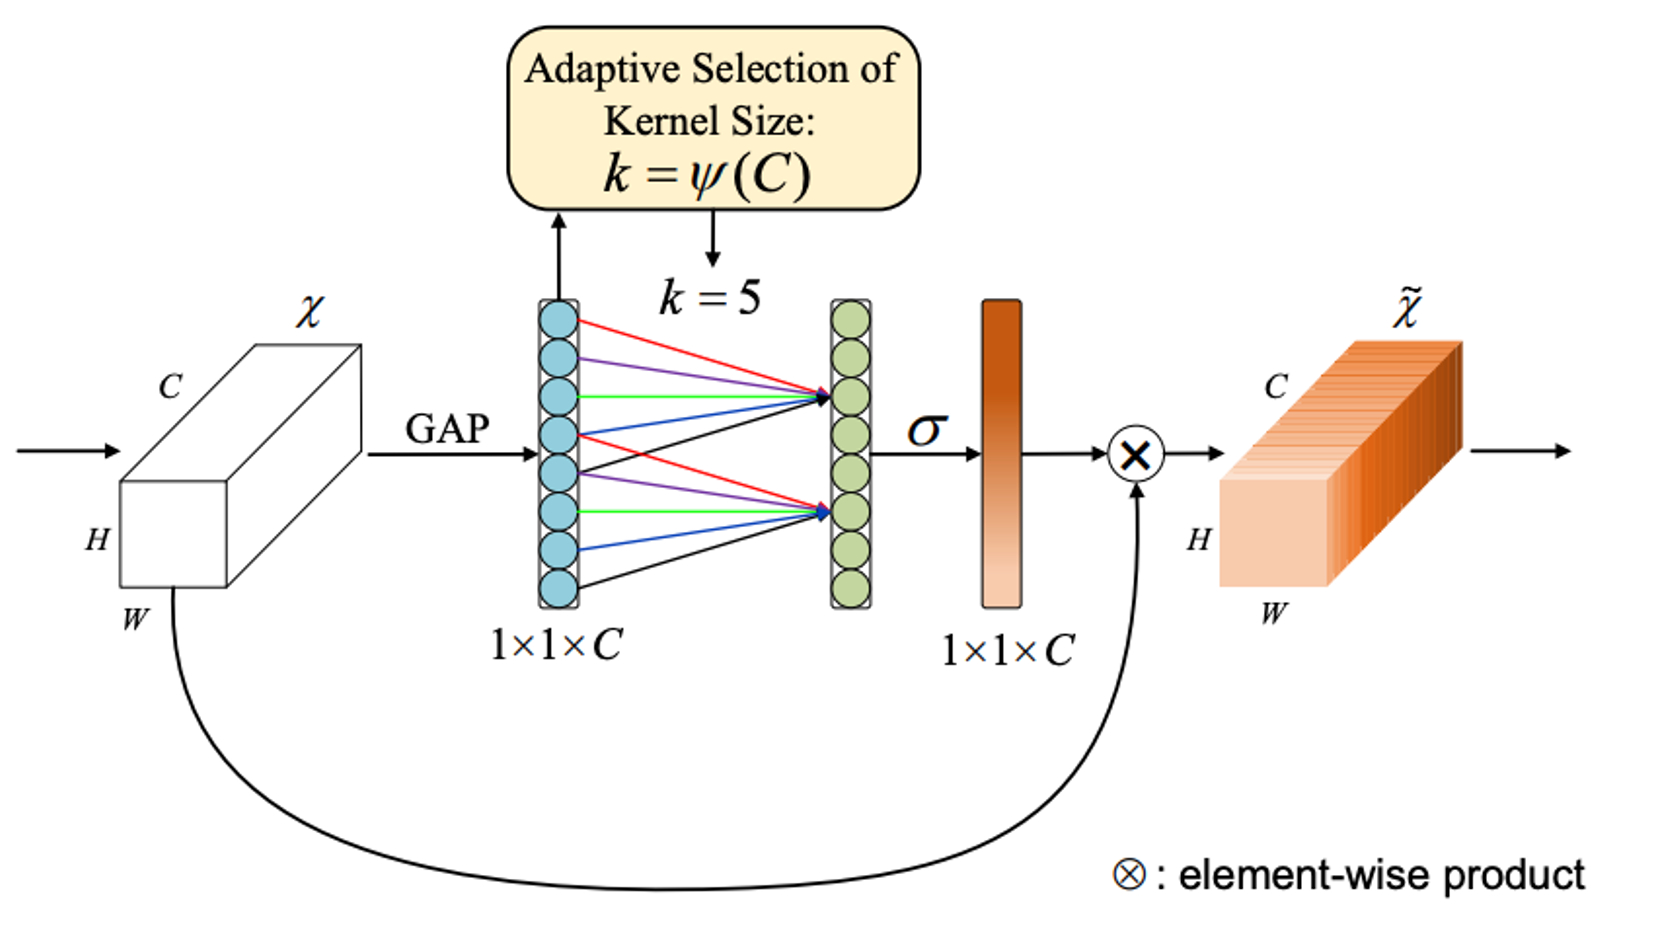
\includegraphics[width=\linewidth]{Fig/ECA.png}
        \caption{Efficient channel attention (ECA) module}
        \label{ecamodule}
\end{figure}

This integration not only enhances the model's ability to capture and utilize multi-scale features effectively but also optimizes the allocation of computational resources. The resulting synergy between attention mechanisms enhances the model's capacity to discriminate and count objects in crowds, making it suitable for diverse scenarios and challenging real-world conditions. By applying an ECA block to each of the layers 3, 4, and 5, we create a robust, flexible, and efficient crowd counting model that excels in various scenarios.

Following the synthesis of features using Bidirectional Feature Pyramid Network (BiFPN), we proceed by transmitting information through the Multi-Scale Conv Attention (MSCA) module. The MSCA module plays a critical role in enhancing the attention mechanism within the model, particularly focusing on features at different scales within the image space. This module consists of convolutional layers that operate at multiple scales simultaneously, enabling the model to capture features ranging from fine details to larger-scale structures within the crowd.

By incorporating MSCA into the model architecture, we ensure that the model optimally allocates attention across different scales, thereby improving its accuracy in crowd counting tasks. This module not only enhances the model's capability to recognize objects at various scales but also complements the multi-level nature of the BiFPN, further refining the model's feature representation and attention mechanism across the entire image.

The combination of BiFPN, MSCA, and ECA creates a multi-directional, powerful, and flexible model architecture. This combination not only enhances representational capabilities but also optimizes attention and object recognition at every detail and scale in the image, making the model particularly suitable for the crucial task of crowd counting.

\subsubsection{\textbf{Density Map Estimator (DME)}}
Following the aggregation and synthesis of essential features from various VGG layers by the Bi-directional Feature Pyramid Network (BiFPN), our focus shifts to the Density Map Estimator (DME) layer—a pivotal element influencing the accuracy of the density map. Structuring the DME layer is as shown in Figure \ref*{fig:2}, not only showcases flexibility but also maximizes the utilization of information from BiFPN's output layers, rendering the crowd counting process more robust and versatile than ever.



\captionsetup[subfloat]{position=bottom,font={scriptsize,sf}}
\begin{figure}[ht]
        \centering
        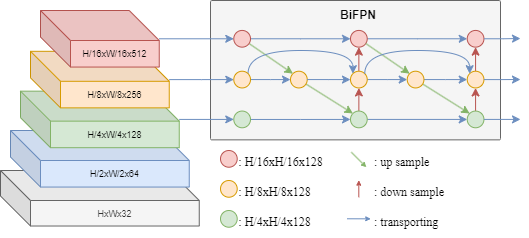
\includegraphics[width=\linewidth]{Fig/BiFPN.png}
        \caption{Bi-directional Feature Pyramid Network}
        \label{BiFPN}
\end{figure}

Connencing with Layer 3 of BiFPN, this layer possesses dimensions H/16 x W/16 (with HxW representing the input image's size). Within each layer, the process encompasses resizing through transposed convolution, information optimization via 3x3 convolutions, and concludes with ReLU activation. Each layer's output comprises 128 channels, concurrently concatenated with the lower BiFPN layer through concatenate to ensure tight interaction and efficiency. Specifically, transposed convolution aims to efficiently restore the size to the original input image dimensions, while the 3x3 convolutional layer adjusts each detail, creating a diverse information space with unique features. This iterative process continues through each subsequent BiFPN layer, progressing from the highest to the lowest. The meticulous tuning of each layer, coupled with astute concatenation from higher to lower layers, enhances the model's flexibility and establishes bidirectional interaction between layers, facilitating the creation of an effective density map amidst crowded objects of varying sizes.

\captionsetup[subfloat]{position=bottom,font={scriptsize,sf}}
\begin{figure}[ht]
        \centering
        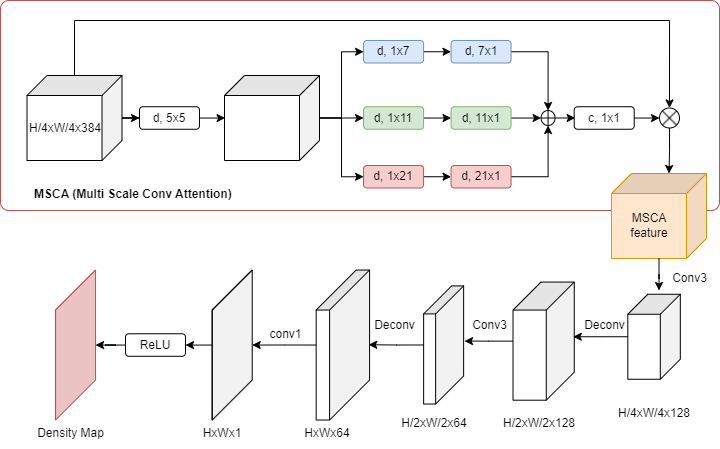
\includegraphics[width=\linewidth]{Fig/densitymapmodule.png}
        \caption{Density Map Estimation Module}
        \label{attentionmap}
\end{figure}

Following three consecutive layers, the outcome is a feature map with 256 channels, and dimensions  H/4 x W/4. To match the input image size (HxW) and reduce channels to 1, we undertake two iterations of transposed convolution and convolution, as depicted in Figure \ref*{fig:2}. Ultimately, the ReLU activation function is applied after the final convolutional layer, as density map values are invariably positive. Consequently, DME generates high-resolution density maps mirroring the input size by amalgamating essential information from the BiFPN block.

\subsection{Density Map Generation}
In a densely populated and crowded scene, each object is represented by three key annotations: $c_i$ (indicating the position), $h_i$ (representing the height), and $w_i$ (indicating the width) for each entity. Each of these parameters holds specific significance in describing the spatial attributes of the objects within the crowd context. The parameter $c_i$ assumes a pivotal role in the accurate determination of the spatial location of each object. It serves as a key factor in establishing the precise coordinates of an object within the given space, enabling a detailed understanding of its position amidst the crowded surroundings. Simultaneously, the values of $w_i$ and $h_i$ contribute to furnishing a holistic perspective on the dimensions of the object. These dimensions collectively provide comprehensive insights into the size and spatial extent of the entities under consideration. Analogous to widely adopted bounding box methodologies in advanced object detection approaches, the combination of $w_i$ and $h_i$ acts as a robust descriptor, encapsulating the object's physical characteristics and facilitating a more nuanced representation within the research framework.

However, the application of object detection and bounding box annotation methods has laid bare certain limitations. Specifically, detection-based model's efficacy encounters challenges in scenarios with overlapping objects, leading to an undesirable increase in inference times for the object detection model\cite{firstdensity}. To address these challenges and enhance the robustness of our approach, we draw inspiration from the groundbreaking research of Zhang et al \cite{mcnn}. In a departure from conventional methods, we advocate for an innovative alternative: the creation of a density map derived from the precise positions of the object specimens, eschewing the direct reliance on point annotations. This strategic shift in approach aims to surmount the constraints associated with overlapping objects and optimize the efficiency of our quantity estimation task.

In a specific instantiation, this alternative approach is implemented on our dataset comprising M trained images denoted as $I_m \{m=1,...,M\}$. Within each image $I_m$, with N objects are annotated, the set of positions $c_i\{i=1,...,N\}$ collectively forms a spatial point map. From This point map 2D, and drawing inspiration from the seminal work of Victor Lempitsky and Andrew Zisserman \cite{firstdensity}, serves as the foundational basis for formulating a density map. Specifically, the authors employ a 2D Gaussian kernel filter expressed as follows:

\begin{equation}
        G_{xy} = \frac{1}{2\pi\sigma^2}e^{-\frac{x^2+y^2}{2\sigma^2}}
        \label{eq: 3}
\end{equation}

In this equation, $G_{xy}$ symbolizes the normalized 2D Gaussian kernel with a variance $\sigma$ and mean value at the position $c_i$. Then, at each position of an annotated object in the image, it is substituted with a normalized 2D Gaussian kernel as delineated in Figure \ref*{fig:1}. Due to the normalization of the Gaussian kernel, information pertaining to both the position and the aggregate number of objects in the image is conserved. Nonetheless, it becomes evident that this methodology has foregone details regarding the size of each individual object. For instance, certain studies tends to designate sigma as a constant, resulting in uniform outputs upon traversal through the Gaussian filter for objects of distinct sizes, thereby relinquishing size-specific information. This method ostensibly demonstrates efficacy only in scenarios wherein object sizes are presupposed to be uniform.

On the other hand, similar to the fixed $\sigma$ approach, within the context of maintaining homogeneity in object sizes, methodologies posited by select papers \cite{hu2022deep,mcnn} deploy dynamic $\sigma$ predicated on the average distance between nearest k-neighbors of objects. This approach presupposes that the spatial distance between an object and its contiguous counterparts dictates its size within the image. However, this solution exhibits suboptimal generalization across diverse cases. In our specific problem domain, even when the size of an object markedly surpasses that of other entities, It is often overlapped by numerous smaller objects. Consequently, utilizing inter-object distances as a size determinant becomes untenable

Confronted with the complexity due to object size heterogeneity, it is  recognize that conventional methodologies employed are oftentimes deemed suboptimal and deficient in accuracy. Consequently, to attain optimal precision in density estimation, careful consideration of individual dimensions within the subject population is necessary. From this challenge, we propose a methodology to generate a density map while retaining details about the object size, under the assumption that the sigma parameter of the Gaussian kernel is proportional to the size of the object. This approach ensures a more comprehensive evaluation of size diversity density within a densely populated, thereby augmenting the overall accuracy of object population density estimation. Algorithm \ref{alg:density} furnishes pseudocode employed for generating a density map based on the proposed methodology.

Within Algorithm 1, for each annotation $\{c_i,h_i,w_i\}$ within an object population image dataset, we dynamically instantiate a normalized Gaussian kernel for each object, denoted as $G_i$, and $\sigma_i$ represents the variance, and $k_i$ denotes the kernel size. This tailored Gaussian kernel $G_i$ is uniquely assigned to each individual object. Such a approach guarantees that the dataset label, denoted as $L$, preserves crucial information pertaining to the size characteristics of each object as well as information about that location of the object. On the other hands, in specific scenarios where close-up shots of object are taken, the resulting image may cause the object to appear larger compared to the actual image size. Subsequently, as these object undergo Gaussian filtering, the variance of the filter increases dueto the enlarged size of the object . This augmented variance leads to the disappearance of the density map at the this object's location, creating a challengefor generating density map efficiently. To mitigate this issue, our proposed solutioninvolves incorporating a scaling factor, denoted as $\alpha$. This $\alpha$ factor, with a value less than 1, is multiplicatively applied to the variance, effectively controlling the image loss experienced by the object during the Gaussian filtering process. Through systematic experimentation, weobserved that setting the $\alpha$ value to 0.5 yielded the most favorable outcomes, demonstrating its efficacy in addressing the challenge posed by excessive variance during image processing.

\begin{algorithm}[H]
        \caption{Algorithm generates a density map by applying a Scale-Adaptive Gaussian Kernel filter}
        \label{alg:density}
        \begin{algorithmic}[1]
                \renewcommand{\algorithmicrequire}{\textbf{Input:}}
                \renewcommand{\algorithmicensure}{\textbf{Output:}}
                \REQUIRE $N$ annotations: $\{c_i,h_i,w_i\}$
                \ENSURE  Output label $L(H \times W)$
                \FOR {$\{c_i,h_i,w_i\}$ in N annotations}
                \STATE $\sigma_i \leftarrow \alpha\sqrt{h_i \cdot w_i}$
                \STATE $k_i \leftarrow 2\sigma_i$
                \FOR {$x \leftarrow 0$ to $k_i$}
                \FOR {$y \leftarrow 0$ to $k_i$}
                \STATE $g_{xy} \leftarrow \frac{1}{2\pi\sigma_i^2}e^{-\frac{(x-\frac{k_i}{2})^2+(y-\frac{k_i}{2})^2}{2\sigma_i^2}}$
                \ENDFOR
                \ENDFOR
                \STATE $G[x,y] \leftarrow
                        {\begin{bmatrix}
                                        g_{00} & g_{01} & \cdots & g_{0k} \\
                                        g_{10} & g_{11} & \cdots & g_{1k} \\
                                        \vdots & \vdots & \ddots & \vdots \\
                                        g_{k0} & g_{k1} & \cdots & g_{kk}
                                \end{bmatrix}}$
                \STATE $G[x,y] = \frac{1}{\sum_{x=0}^{k}\sum_{y=0}^{k}G[x,y]} \cdot G[x,y]$
                \FOR {$x = 0$ to $k$}
                \FOR {$y = 0$ to $k$}
                \STATE $l_i[x+c_i-\frac{k}{2},y+c_i-\frac{k}{2}] = G[x,y]$
                \ENDFOR
                \ENDFOR
                \STATE $L \mathrel{+}= l_i$
                \ENDFOR
                \RETURN $L(H \times W)$
        \end{algorithmic}
\end{algorithm}

\captionsetup[subfloat]{position=top,font={scriptsize,sf}}
\begin{figure}[h]
        \centering
        \subfloat[\label{GenDensity_1a}]{
                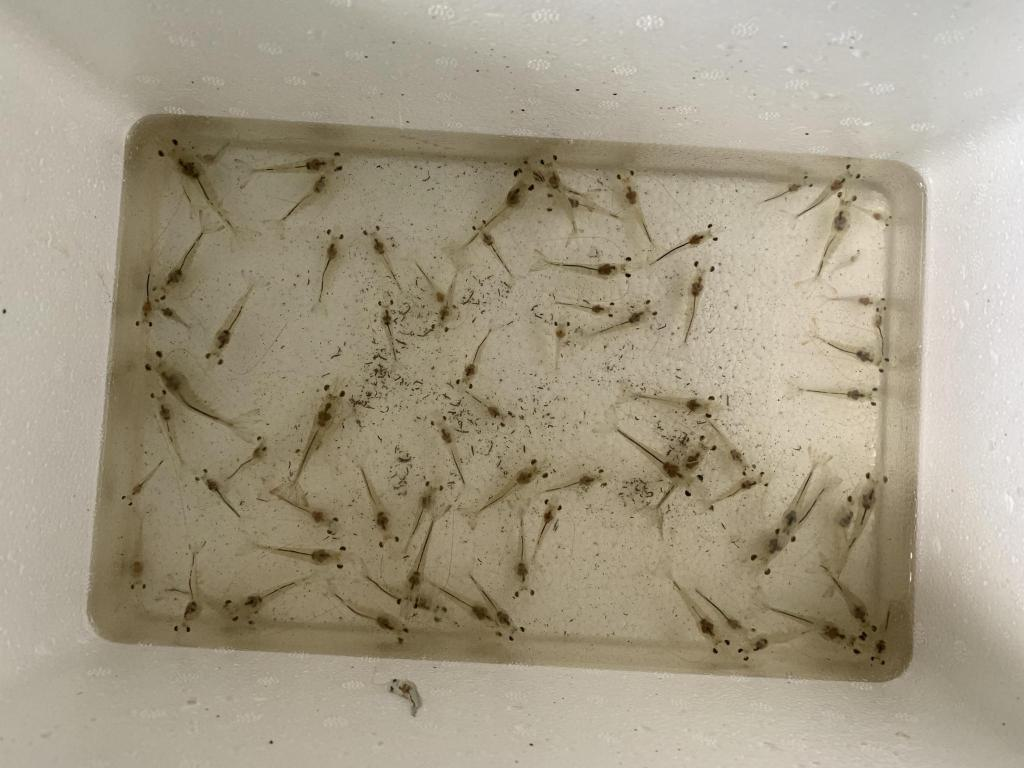
\includegraphics[width=0.235\linewidth]{Fig/328_img.jpg}}
        \subfloat[\label{GenDensity_1b}]{
                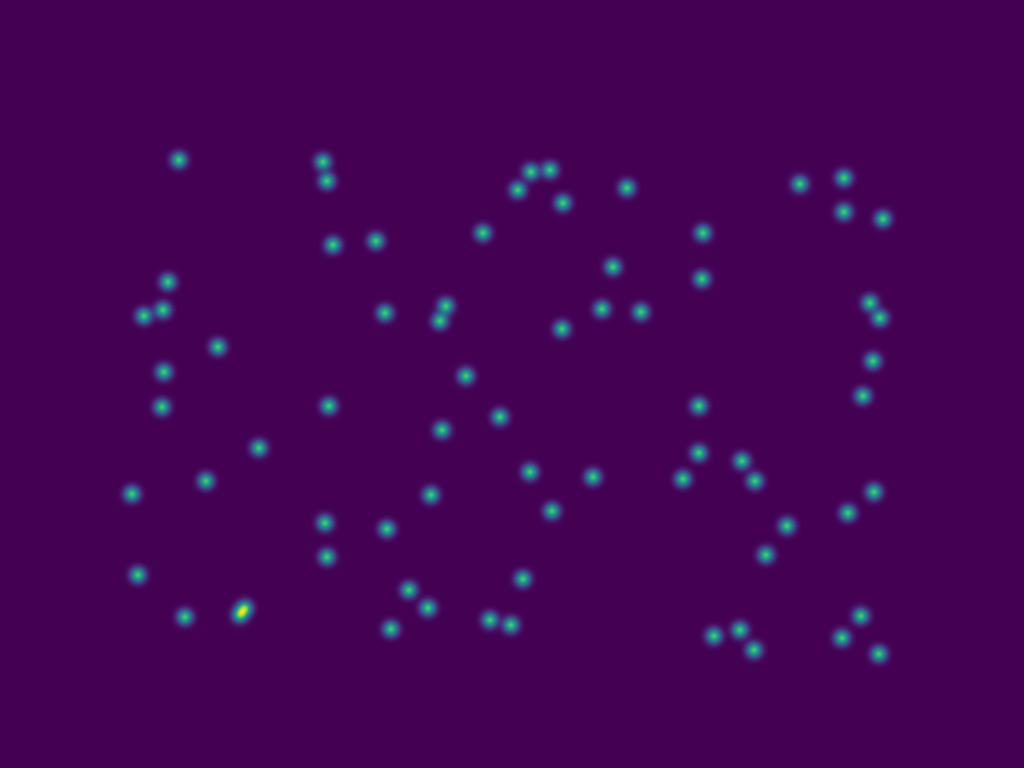
\includegraphics[width=0.235\linewidth]{Fig/328_fix.jpg}}
        \subfloat[\label{GenDensity_1c}]{
                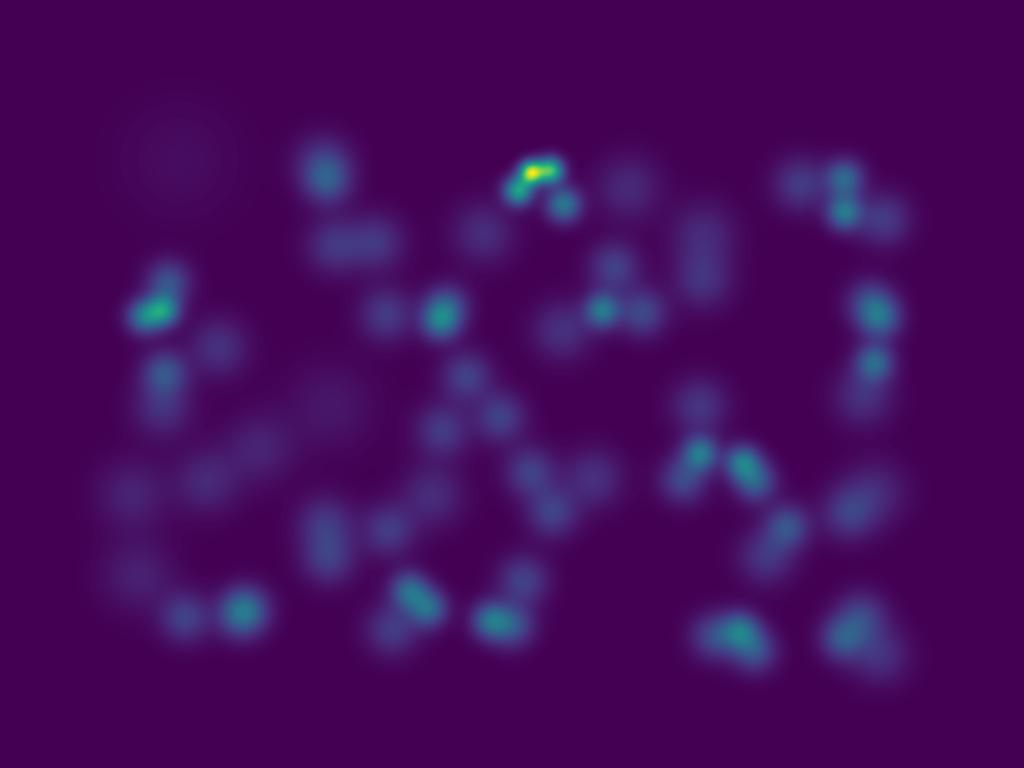
\includegraphics[width=0.235\linewidth]{Fig/328_adap.jpg}}
        \subfloat[\label{GenDensity_1d}]{
                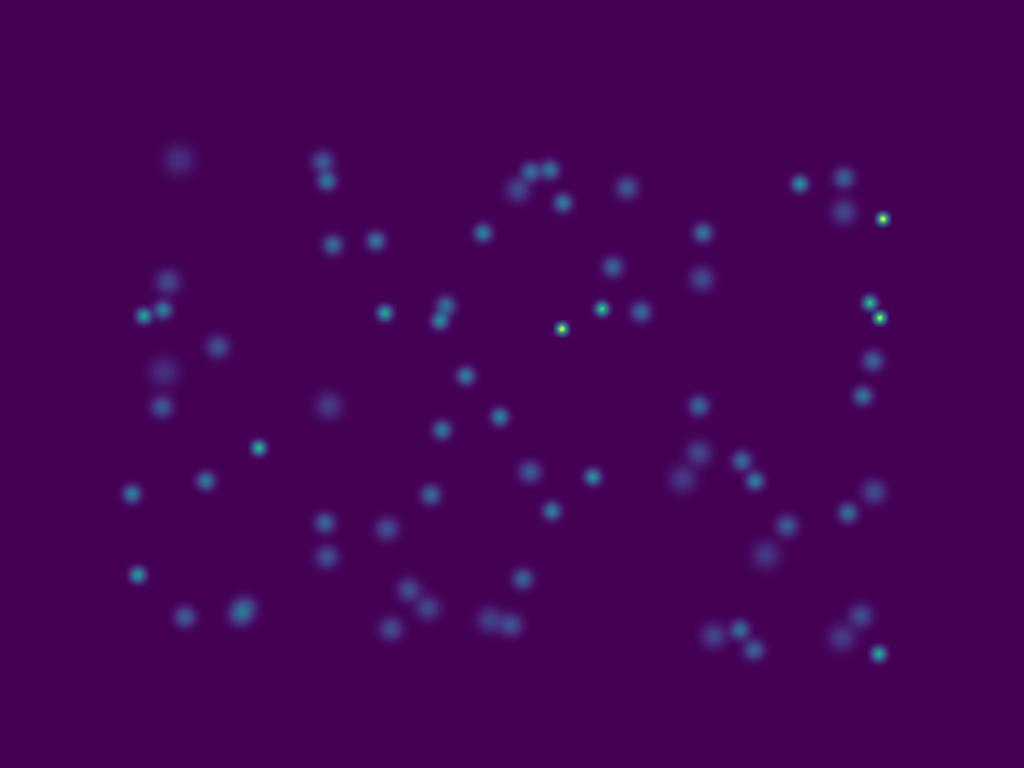
\includegraphics[width=0.235\linewidth]{Fig/328_size.jpg}}
        \\
        \subfloat{
                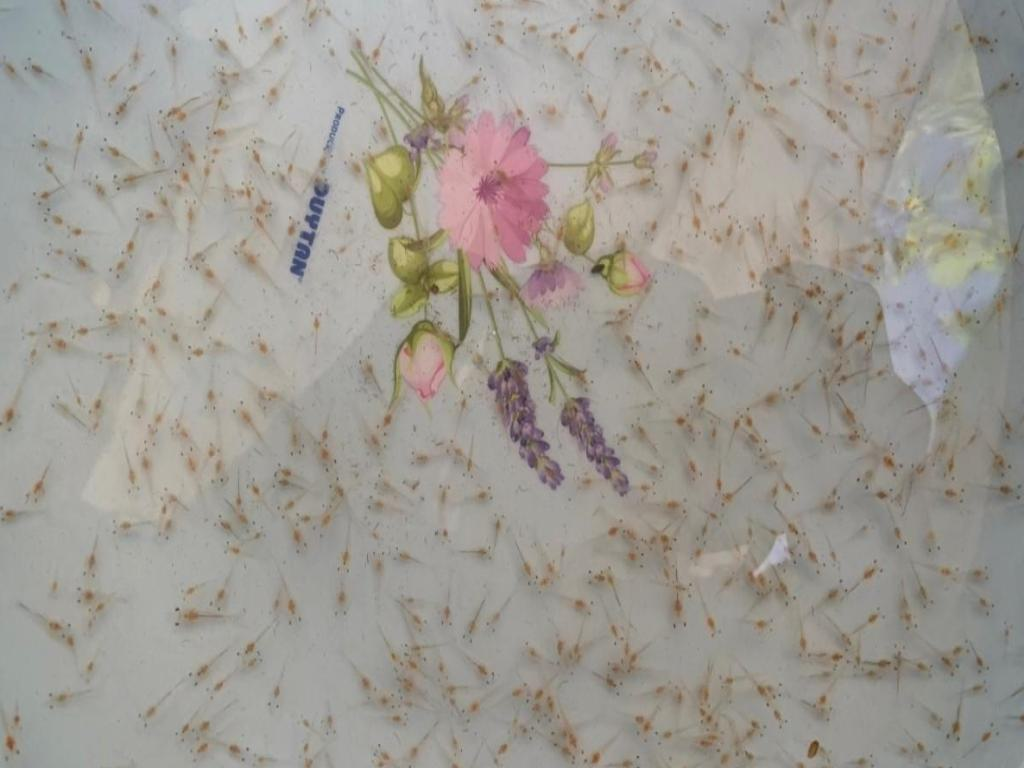
\includegraphics[width=0.235\linewidth]{Fig/204_img.jpg}}
        \subfloat{
                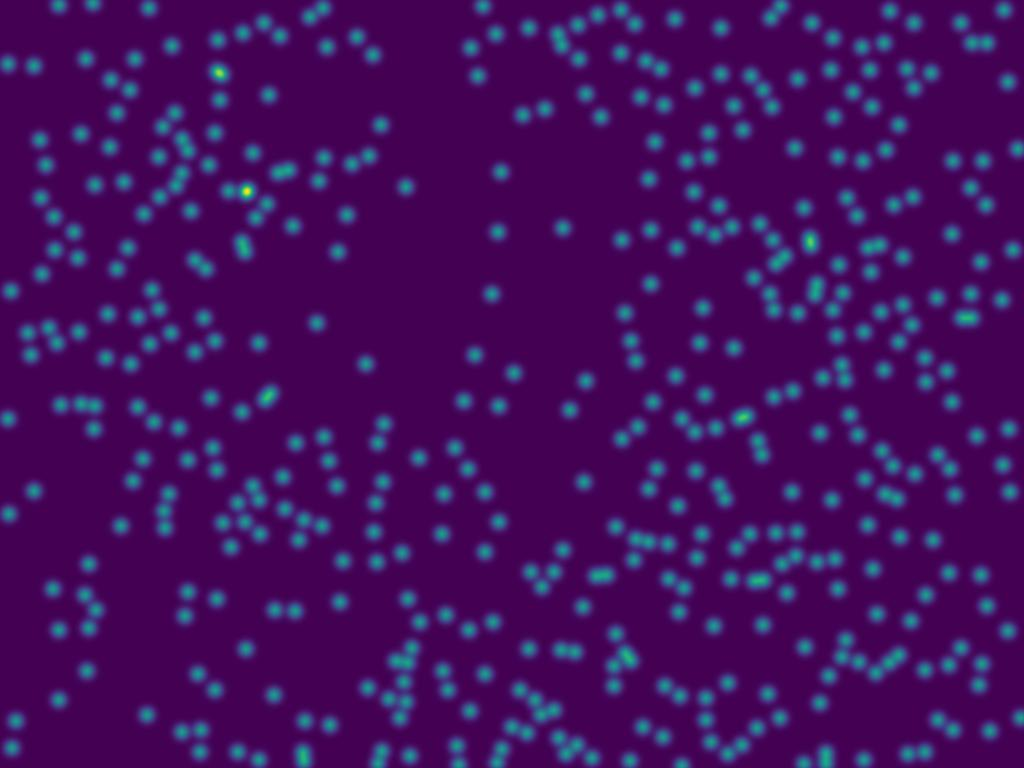
\includegraphics[width=0.235\linewidth]{Fig/204_fix.jpg}}
        \subfloat{
                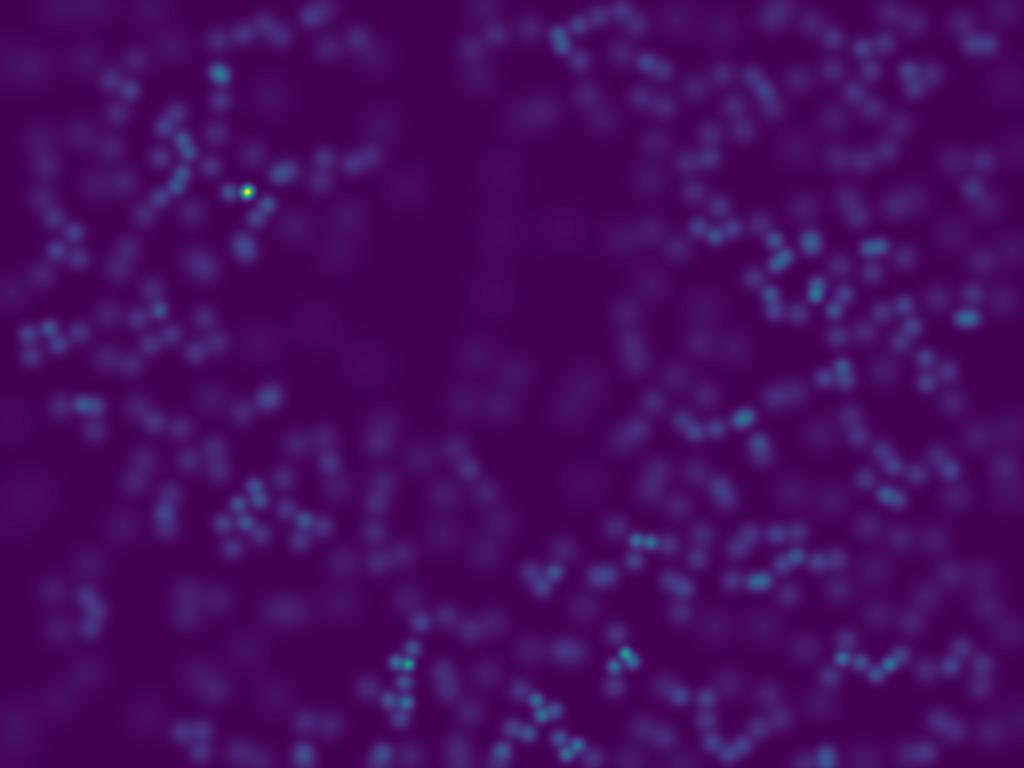
\includegraphics[width=0.235\linewidth]{Fig/204_adap.jpg}}
        \subfloat{
                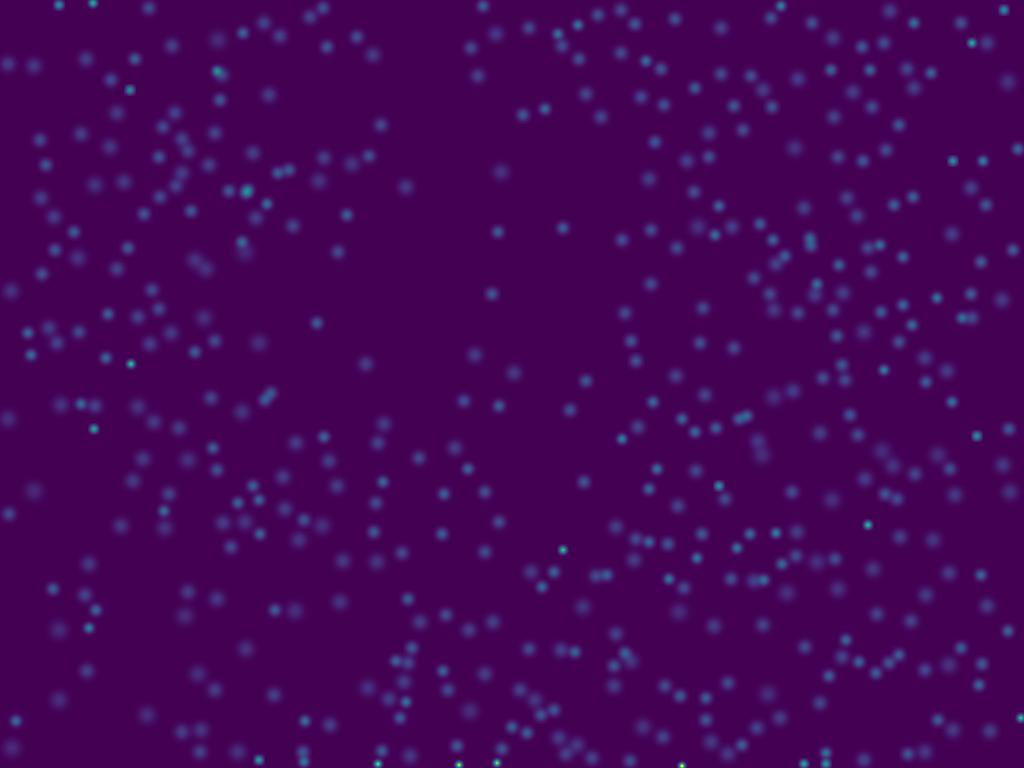
\includegraphics[width=0.235\linewidth]{Fig/204_size.jpg}}
        \caption{Generate a depth map by applying the Gaussian kernel. (a) Original image of shrimp larvae, (b) Density map applying Gaussian kernel with constant $\sigma$, (c) Density map is generated applying Gaussian kernel with dynamic $\sigma$ based on the average k-nearest neighbor distance, (d) Density map is generated applying Gaussian kernel with dynamic $\sigma$ based on size}
        \label{fig:1}
\end{figure}
\section{Experiments Evaluation}
\subsection{Acquisition of Datasets}

\begin{table}[ht]
        \centering
        \caption{Number of Shrimp Larvae}
        \begin{tabular}{l|cc}
            \toprule
            Number of Shrimp larvae & Number of images\\
            \midrule
            under 100                   & 2647    \\
            between 100 and 200         & 1443    \\
            between 200 and 300         & 448    \\
            between 300 and 400         & 194    \\
            between 400 and 500         & 140    \\
            between 500 and 600         & 32    \\
            between 600 and 700         & 115    \\
            Total                       & 5019    \\

            \bottomrule
        \end{tabular}
    \end{table}

Our study is centered around the intricate task of estimating the quantity of objects present in images under conditions that involve a complex mixture of objects with varying dimensions. The paramount challenge we address is the inherent diversity in the sizes of these objects. Consequently, identifying and characterizing objects with heterogeneous size distributions becomes a critical aspect of our research.

The focus on shrimp larvae as our chosen subjects is grounded in their inherent characteristics.  The rapid and disparate growth rates among individuals within a group of larvae create a scenario where the size of one sample can significantly exceed that of another within the same population as shown in Figure \ref*{fig3}. This variability underscores the need for an innovative approach to object detection and counting, particularly in dynamic environments such as aquaculture facilities.

Our adoption of a supervised learning methodology necessitates the availability of annotated datasets, a pivotal component in training our model. To ensure the relevance and authenticity of our data, we meticulously collected segmented videos in a systematic manner during on-site filming at various aquaculture facilities. This rigorous approach is designed to replicate the complexities of real-world shrimp production environments, reinforcing the robustness and applicability of our experimental results.

In pursuit of a model that thrives in practical deployment scenarios, we executed a comprehensive video recording strategy. This involved capturing multiple videos under diverse conditions, including alterations in camera angles, variations in lighting parameters, and fluctuations in both the quantity and size of shrimp populations within the tanks. Our intention is to create a dataset that encapsulates the intricacies of the shrimp farming milieu, ensuring that our model is well-equipped to handle the challenges posed by real-world scenarios.

From the extensive library of recorded videos, we meticulously extracted images by adopting a sampling approach, selecting one frame every 60 frames from each recorded shrimp video. This process generated a substantial collection of images that served as the foundation for our subsequent analyses.

The next crucial step in our methodology involved annotating each image to facilitate effective utilization of the supervised learning approach. A key consideration was the level of annotation required. Recognizing the natural inclination of humans to count objects, we deemed point annotation as an indispensable feature in our dataset. Furthermore, the annotation of object sizes emerged as another critical aspect of our research. Each object within the frame was meticulously annotated with three parameters: $xi$ (position), $wi$ (width), and $hi$ (height), providing a holistic representation of the object in question.

\captionsetup[subfloat]{position=bottom,font={scriptsize,sf}}
\begin{figure}[h]
        \centering
        \subfloat[\label{fig3_a}]{
                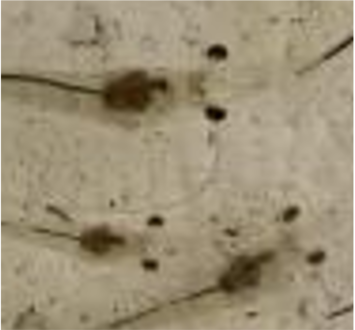
\includegraphics[width=0.3\linewidth]{Fig/origin image.png}}
        \subfloat[\label{fig3_b}]{
                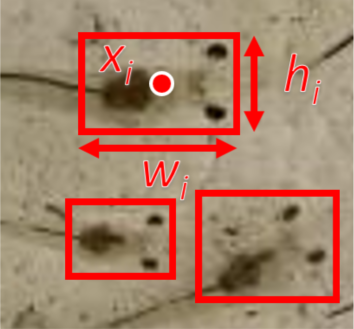
\includegraphics[width=0.3\linewidth]{Fig/boundingbox.png}}
        \subfloat[\label{fig3_c}]{
                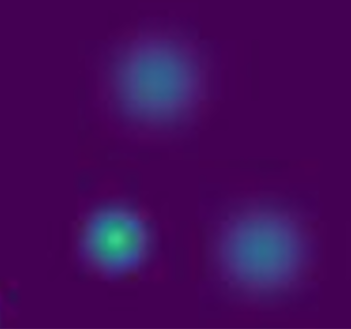
\includegraphics[width=0.3\linewidth]{Fig/densitymap.png}}
        \caption{(a): Original image, (b) Annotated image, (c) Density map generated by Size-Adjustable Gaussian Kernel. We annotated three kinds of keypoints on each larva from their bound box: $c_i$, $h_i$ and $w_i$ correspond to the center, height and width of the bounding box. }
        \label{fig3}
\end{figure}

\subsection{Evaluation Metric}
In this study, we employ two pivotal metrics to gauge the predictive prowess of the model: Mean Absolute Error (MAE) and Mean Squared Error (MSE).

MAE is expressed by the following formula:

\[
\text{MAE} = \frac{1}{N} \sum_{i=1}^{N} \left| y_i - \hat{y}_i \right|
\]

Here, \( N \) represents the number of samples, \( y_i \) denotes the ground truth value, and \( \hat{y}_i \) signifies the predicted value. MAE quantifies the average absolute difference between predicted and actual values of the crowd size.

MSE is computed using the formula:

\[
\text{MSE} = \frac{1}{N} \sum_{i=1}^{N} \left( y_i - \hat{y}_i \right)^2
\]

This formula calculates the average squared difference between predicted and actual values. The incorporation of both MAE and MSE allows for a comprehensive assessment of the model's accuracy and sensitivity in the context of crowd counting, offering valuable insights into various types of prediction errors. We anticipate that this amalgamation will streamline the evaluation process and elevate the model's performance in real-world applications.

\subsection{Evaluation and Comparison}
\begin{table}[ht]
        \centering
        \caption{Performance Comparison of Different Methods}
        \begin{tabular}{l|ccccccc}
            \toprule
            \multirow{2}{*}{Method} & \multicolumn{3}{c}{MAE} & \multicolumn{3}{c}{RMSE} \\ \cmidrule(lr){2-4} \cmidrule(lr){5-7}
            & Fix & k-NN & Scale & Fix & k-NN & Size \\
            \midrule
            CAN         & 14.44 & 17.88 & 10.37 & 17.52 & 22.18 & 13.05 \\
            CFFNet      & 19.99 & 27.45 & 13.91 & 23.71 & 32.38 & 17.18 \\
            CSRNet      & 12.06 & 17.67 & 13.23 & 14.58 & 22.33 & 16.76 \\
            SANet       & 10.77 & 36.3  & 11.91 & 13.6  & 43.05 & 14.59 \\
            TEDNet      & 11.55 & 19.89 & 11.08 & 14.61 & 24.74 & 13.73 \\
            SGANet      & 36.69 & 43.38 & 20.2  & 39.93 & 52.55 & 25.25 \\
            Ours Model  & 12.59 & 18.99 & 9.81  & 16.05 & 23.6  & 12.77 \\
            \bottomrule
        \end{tabular}
    \end{table}

We compared our proposed model with several state-of-the-art methods for crowd counting and density estimation, including CAN, CFFNet, CSRNet, SANet, TEDNet, and SGANet. Each of these methods employs different strategies for handling object counting, offering a diverse set of benchmarks against which to assess our approach.

The results of our experiments, as presented in Table II, clearly demonstrate the superior performance of our model. Our method achieves a significantly lower MAE and MSE compared to the other approaches, indicating higher accuracy and robustness in object counting. This improvement can be attributed to the effectiveness of our Size-Adjustable Gaussian Kernel in capturing object size variations and generating accurate density maps, along with the powerful feature extraction and attention mechanisms incorporated within our CNN architecture.

Moreover, we also delved deeper into the performance of various models under different conditions related to object size handling. We specifically examined three scenarios: using a fixed Gaussian kernel (Fix), a kernel with dynamic sigma based on k-nearest neighbors (k-NN), and our proposed Size-Adjustable Gaussian Kernel (Scale). This analysis provided valuable insights into the strengths and weaknesses of each approach.

Fixed Kernel (Fix): Models employing a fixed Gaussian kernel with constant sigma exhibited the lowest accuracy across the board. This approach, while simple, fails to account for the diverse sizes of objects within the dataset. Consequently, the generated density maps were less accurate, leading to higher MAE and MSE values for all models.

k-Nearest Neighbors (k-NN): Utilizing a dynamic sigma based on the average distance between k-nearest neighbors showed some improvement over the fixed kernel approach. This method attempts to adapt to size variations by considering the local density around each object. However, it still falls short of capturing individual object sizes accurately, particularly in cases where objects overlap significantly or exhibit large size discrepancies. As a result, while k-NN models demonstrated better performance than those with fixed kernels, their accuracy remained inferior to our proposed method.

Size-Adjustable Gaussian Kernel (Size): Our proposed approach, employing a Size-Adjustable Gaussian Kernel, consistently outperformed the other methods across all models. By dynamically adjusting the kernel parameters based on individual object dimensions, we ensured that the generated density maps accurately reflect the size variations within the population. This led to a significant reduction in both MAE and MSE, demonstrating the superior accuracy and robustness of our method.

\section{Conclusion}
This paper presented a novel approach for object counting, specifically addressing the challenges posed by diverse object sizes and dense scenarios. Our proposed method, utilizing a Size-Adjustable Gaussian Kernel for density map generation, effectively incorporates individual object size information, leading to significant improvements in counting accuracy compared to existing methods.

Besides, the integration of the BiFPN architecture and attention mechanisms, such as ECA and MSCA, within our CNN model further enhanced feature extraction and object recognition across different scales. Extensive experiments on a challenging shrimp larvae image dataset confirmed the efficacy of our approach, showcasing its ability to handle size variations and dense clusters effectively.

The superior performance of our model paves the way for more precise and reliable object counting in various applications, including crowd analysis, traffic monitoring, ecological surveys, and industrial quality control. Future work could explore incorporating additional object features, such as shape or texture, into the density map generation process and investigating the application of our method to other object counting tasks with similar challenges.
\bibliographystyle{IEEEtran}
\bibliography{bibliography.bib}


\newpage

\vfill

\end{document}


